\section{Method}
\label{sec:method}

\begin{figure}[H]
    \caption{Project Flowchart}
    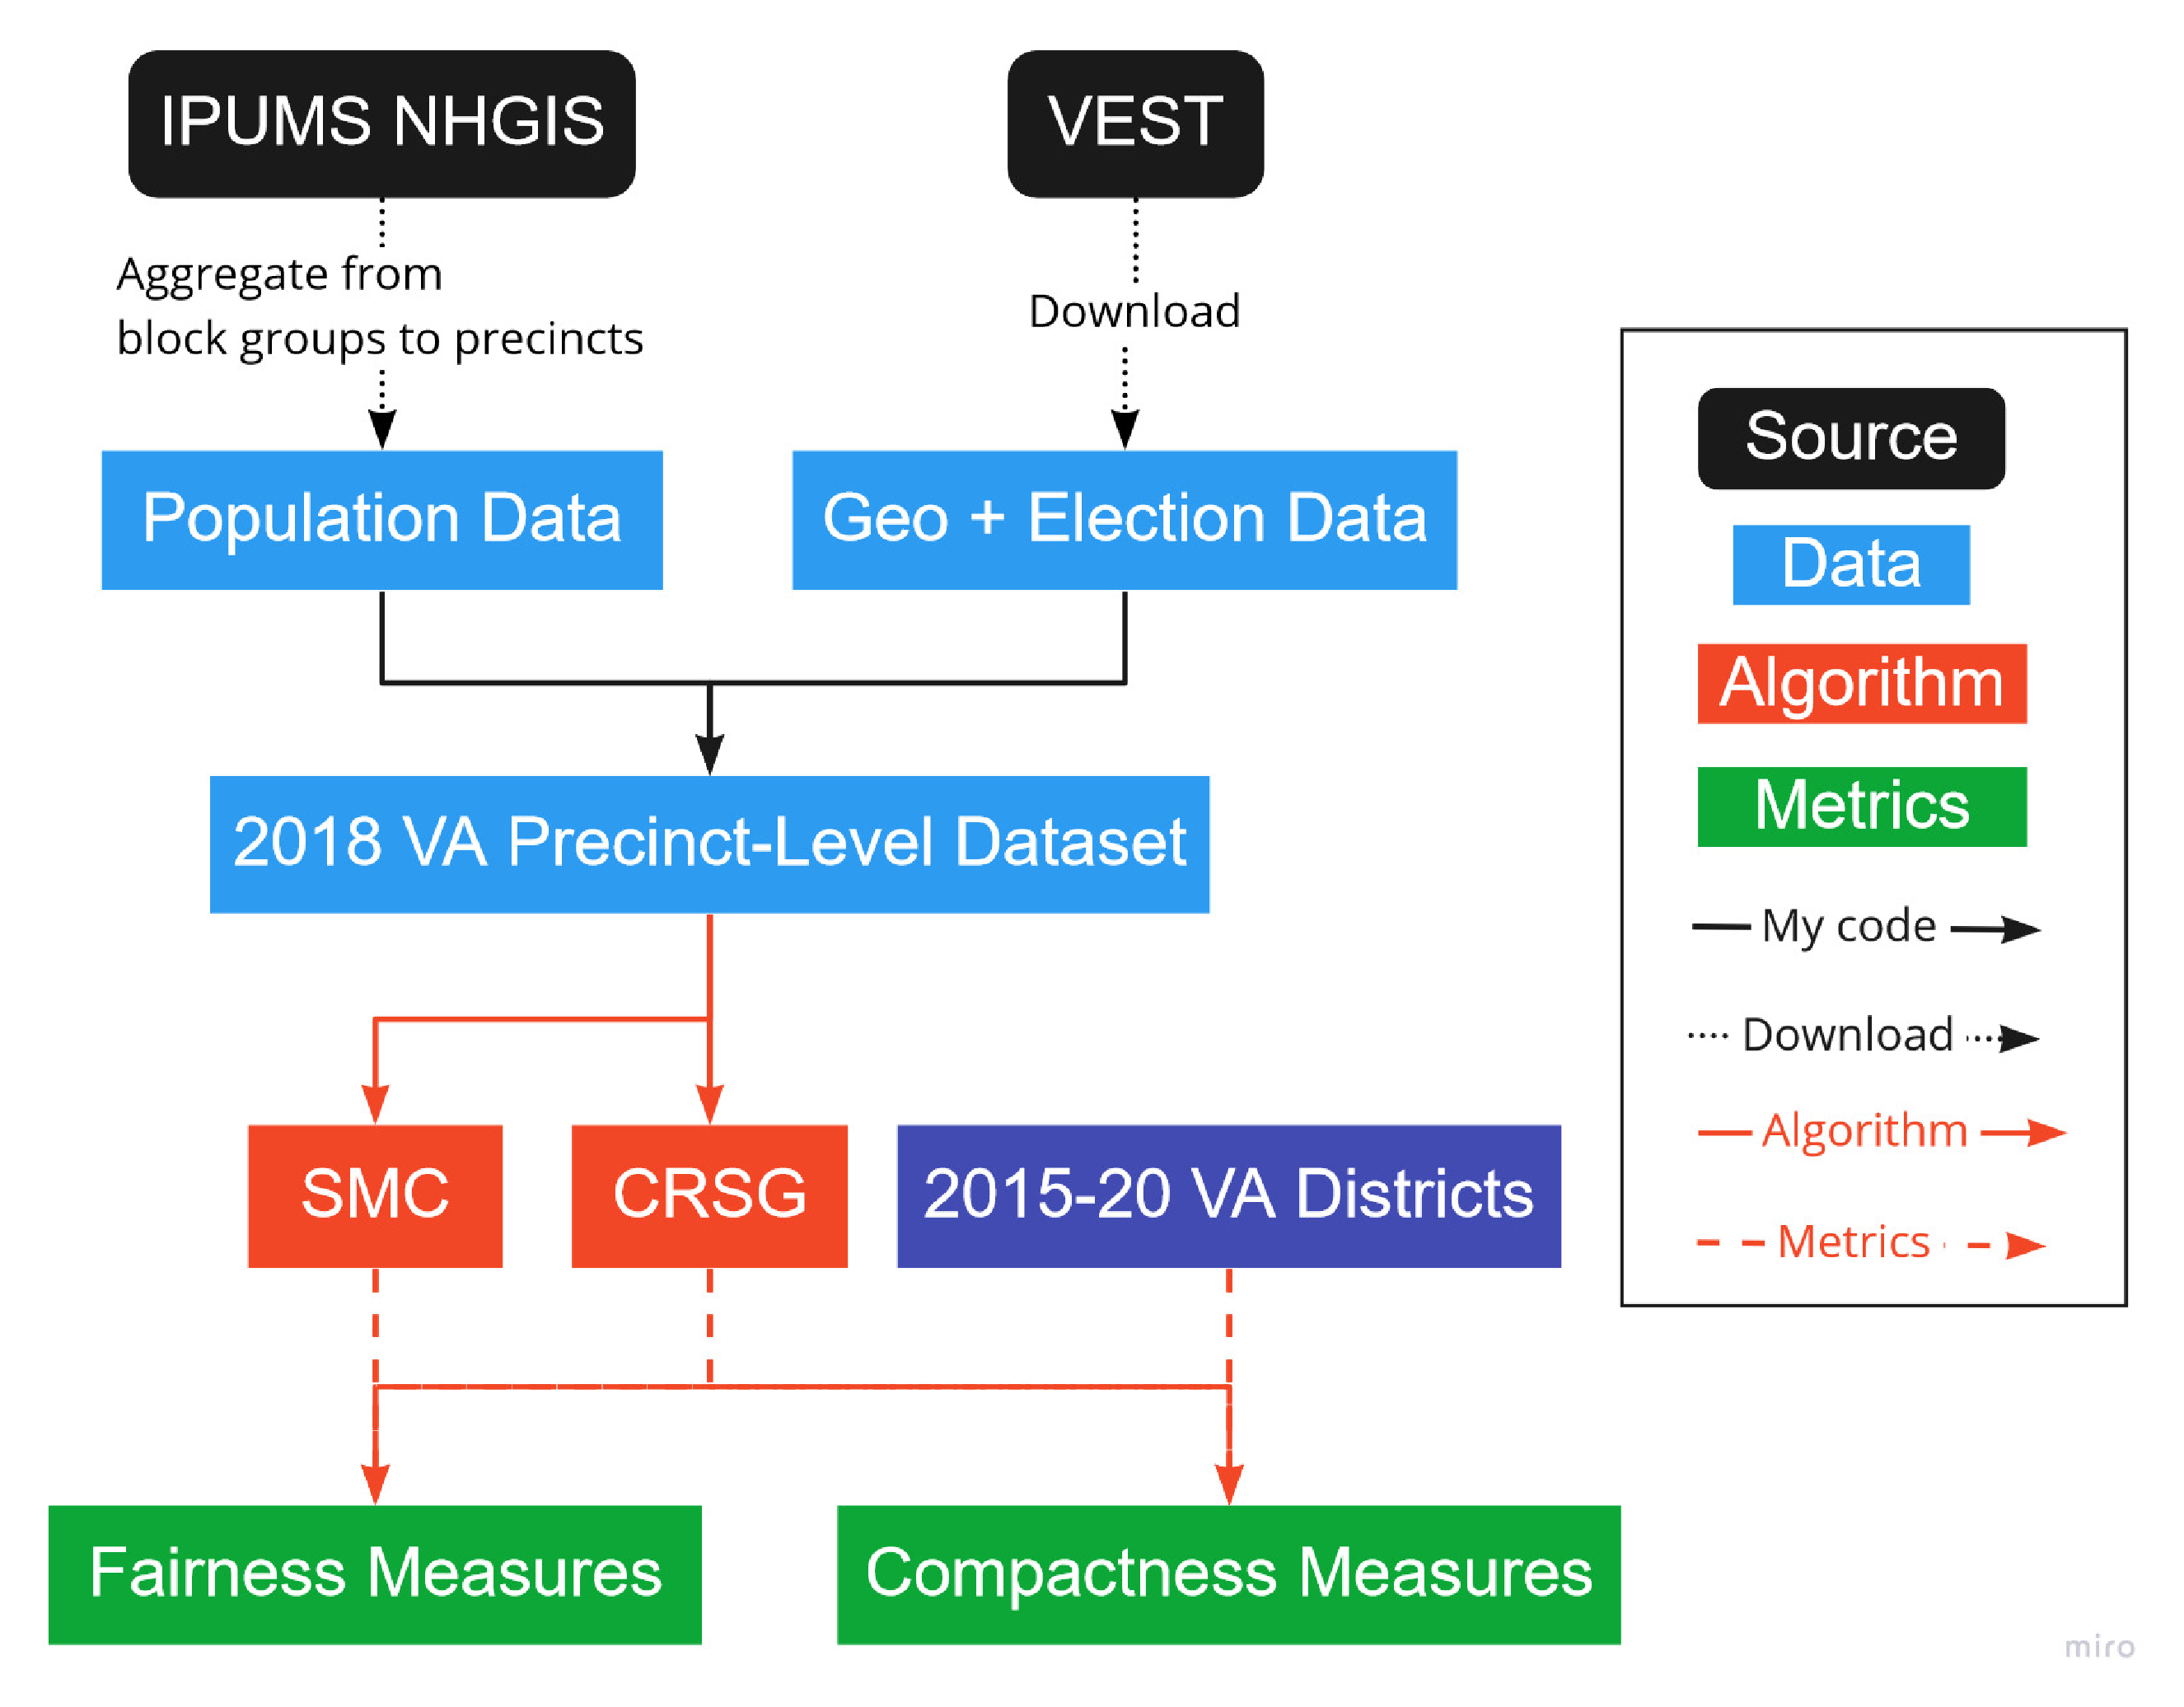
\includegraphics[width=0.85\linewidth]{img/flowchart.pdf}
    \label{fig:flowchart}
    \raggedright
    \figurenote{Black, blue, purple, red, and green correspond to sources, data, the control, algorithms, and metrics, respectively.}
\end{figure}  

My research method simulates the 2021 redistricting of the congressional districts in Virginia using two different algorithms supplied with data from 2018. Figure \ref{fig:flowchart} provides an overview of this process.

\subsection{Choice of Research Focus}

I chose Virginia as my case state because 
\begin{seriate}
    \item it has had to redistrict mid-decade due to gerrymandering \parencite[see][]{wittmanvpersonhuballah2016},
    \item it is a competitive state from an electoral perspective \parencite{virginiadeparmentofelections2021}, 
    \item it recently approved a constitutional amendment that institutes a redistricting process driven by a hybrid commission \parencite{ballotpedia2020}, and
    \item it has a complex geography.
\end{seriate}

With the goal of comparing the performance of different automated redistricting algorithms, I chose two algorithms of different levels of complexity that could both meet the real-world requirements of equal population and compactness. The \hyperref[sec:crsg]{CRSG} \parencite{chen2013} and the \hyperref[sec:smc]{SMC} \parencite{mccartan2020} algorithms were chosen as they both satisfy the aforementioned requirement, are implemented by an open-source software package \parencite{fifield2020d}, and together they represent the evolution in the scholarship on such algorithms. 

Since there is no single measure of partisan fairness nor compactness agreed upon by the scholarship \parencite{katz2020}, I selected representative samples of the different perspectives on each measure. For compactness, one geometry-based measure (the \hyperref[sec:polsbypopper]{Polsby-Popper} score) and one graph-theory-based measure (the \hyperref[sec:edgecut]{edge-cut compactness} score) were chosen. For partisan fairness, the simulated election measure (the \hyperref[sec:seatsvotes]{seats-votes curve}) and four single-valued fairness measures (\hyperref[sec:bias]{partisan bias}, the \hyperref[sec:effgap]{efficiency gap}, \hyperref[sec:declination]{declination}, and the \hyperref[sec:meanmed]{mean-median difference}) were chosen. Together, these five partisan fairness measures represent differing and disputed views on how "fairness" should be quantified \parencite{katz2020}. 

\subsection{Choice of Research Method}

I chose the experimental design method because it allowed me to isolate the impact of the redistricting algorithm on map quality from possible confounding variables. This method also includes the use of a control group, which allows the researcher to establish causation. \parencite{peirce2014}

\subsection{Components of Experimental Design}

The experimental unit is the complete dataset (with geographic, population, and election data) for 2018 in Virginia. Every row in each dataset corresponds to a precinct, the smallest geographical unit by which votes are tabulated in Virginia. For each precinct, I also have the total population and the number of votes cast for the 2018 Democratic and Republican candidates. Additionally, each precinct has a polygon associated with it that represents its geographical shape.

The treatments  are the two different redistricting algorithm that I'm comparing: SMC and CRSG. I'm using the implementations in the R programming language "redist" package v2.0-2 \parencite{fifield2020d}. The algorithms were chosen because they represent an evolution in the design of algorithms within the scholarship while still meeting the equal population and compactness requirements.

The response variables are the compactness and partisan fairness measures that I outlined in the \hyperref[sec:litreview]{Literature Review}. This includes the Polsby-Popper score, the edge-cut compactness measure, the seats-votes curve, partisan bias, the efficiency gap, declination, and the mean-median difference. Each measure is computed for each map generated by each algorithm.

The control group is the official Virginia Congressional district map from 2016-2020. I compute the same metrics for this map as for the maps generated by the algorithms.

\subsubsection{Principles of Experimental Design}

Every experimental unit will receive each treatment, and every experimental unit can be replicated many times without issue, so there's no error from a lack of randomization. 

Each algorithm will generate 100 sample redistricting maps. This is large enough to allow for inferences, but small enough to still be computationally feasible. 

All of the redistricting will be happening in controlled environments, so there will be no way for lurking variables to creep in and confound my results. 

\subsection{Data Cleaning}

To create my datasets, I cleaned and compiled three different types of data: demographic data, Geographic Information Systems (GIS) data, and election data.

One required piece of data required to redistrict is demographic data at the precinct level. For my purposes, this means the total population of each precinct. To run the most accurate redistricting simulations, these data needed to be as recent as possible. Comprehensive population counts are only conducted by the US Census Bureau every 10 years, so I instead used the 5-year American Community Survey results at the block-group level. This is a sample survey, not a population count, but that is offset by the aggregation of sample data over a 5 year period. I downloaded this data from the IPUMS National Historic GIS project \parencite{mansonsteven2020}. Using the "maup" Python Library \parencite{hully2020}, I disaggregated the data from the block-group level to the block level, prorating the demographic data based on population. This data was then aggregated up to the precinct level, resulting in a total population count for each precinct.

To redistrict, the algorithms need to know the shape and relative location of each precinct. In practice, this means every precinct has a polygon associated with it and a coordinate reference system that describes where these polygons fall in space. These data tables with the geometry column are known as "shapefiles." I accessed these shapefiles from the Voting and Election Science Team on their Harvard Dataverse \parencite{votingelectionscienceteam2019}. I then merged in my precinct-level demographic data tables to create shapefiles with the necessary demographic data. Since election administrators are free to change the precincts between elections, precinct shapefiles are unique to both a place and a time. I therefore used shapefile data (and demographic and election data) from 2018, the most recent year they were available for.

The last required data type is the count of votes for each party in each precinct. The shapefile dataset from the Voting and Election Science Team already included this data, which was gathered from the Virginia Department of Legislative Services \parencite{votingelectionscienceteam2019}.